\chapter{Introduction to Dart}
Dart is a programming language designed mainly for client development, such as for the web and mobile apps. Developed by Google, it is gaining popularity quite fast and it can also be used to build server and desktop applications.\\
Dart is an Object-oriented, class based, garbage collected language with C like syntax.\\
Dart can either compile to either native code or to JavaScript\\
It supports interfaces, mixins, abstract classes, reified generics, and type inference.\\

\begin{figure}[h]
  \begin{center}
  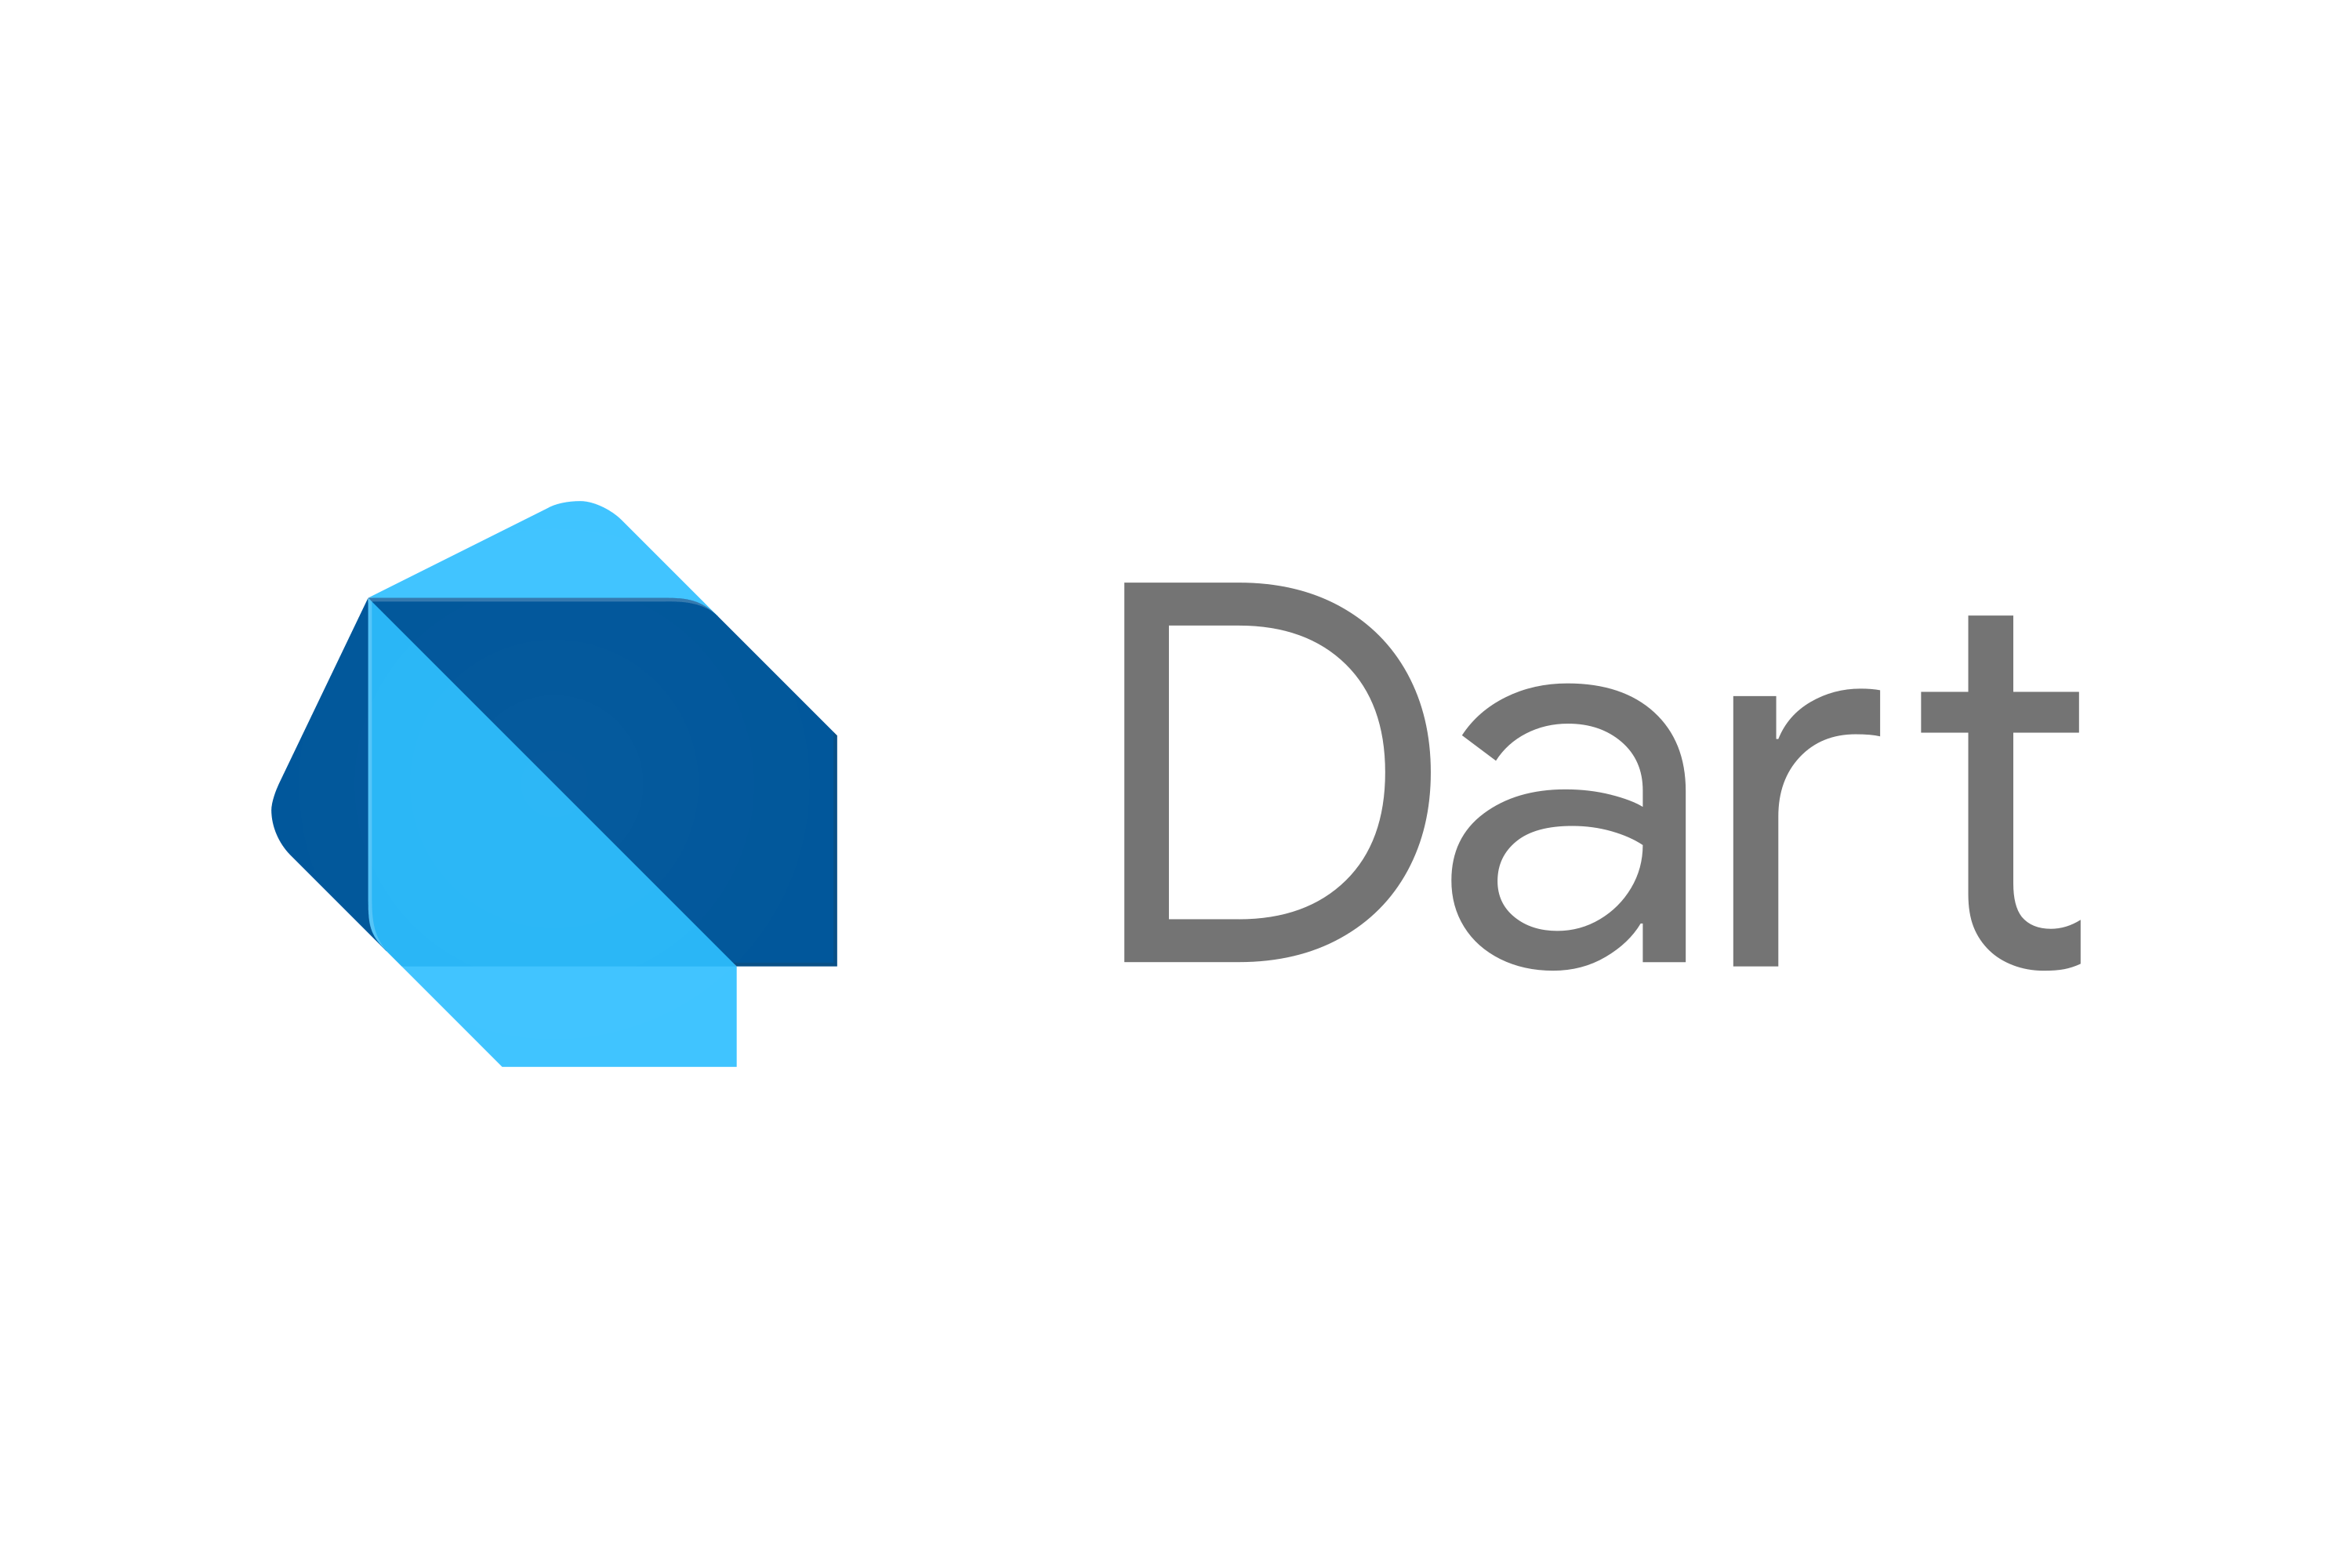
\includegraphics[height=55mm]{Images & Logos/CH02_dart.png}\\
  \end{center}
  \caption{Dart Language}
\end{figure}  

\section{History}
\begin{itemize}
  \item Unveiled at GOTO conference in Aarhus, Denmark, on October 10-12 2012.
  \item The dart project was founded by Lars Bak and Kasper Lund.
  \item Dart 1.0 was released on November 14,2013.
  \item Dart 1.9 released in 2015 to focus on compiling Dart to JavaScript.
  \item Dart 2.0 released in August 2018
  \item Dart 2.6 introduced new extension, dart2native
\end{itemize}

